\documentclass[Arkitektur/System_main.tex]{subfiles}
\begin{document}
\subsection{Logical View}
I dette afsnit præsenteres det logiske view i 4 + 1 modellen. Dette view omhandler funktionaliteten af systemet i forhold til brugeren og hvordan den er struktureret. Funktionaliteten beskrives i afsnittet ved brug af klassediagrammer og state-machines fra applikationsmodellen.

%OPRETTELSE AF BRUGERPROFIL
\subsubsection{Oprettelse af brugerprofil}
For User Sign Up er der lavet et klassediagram, samt et statemachine diagram. Klassediagrammet ses på figur \ref{fig:UserSignUpCD} og statemchine diagrammet på figur \ref{fig:fig:UserSignUpSTM}.
\begin{figure}[H]
    \centering
    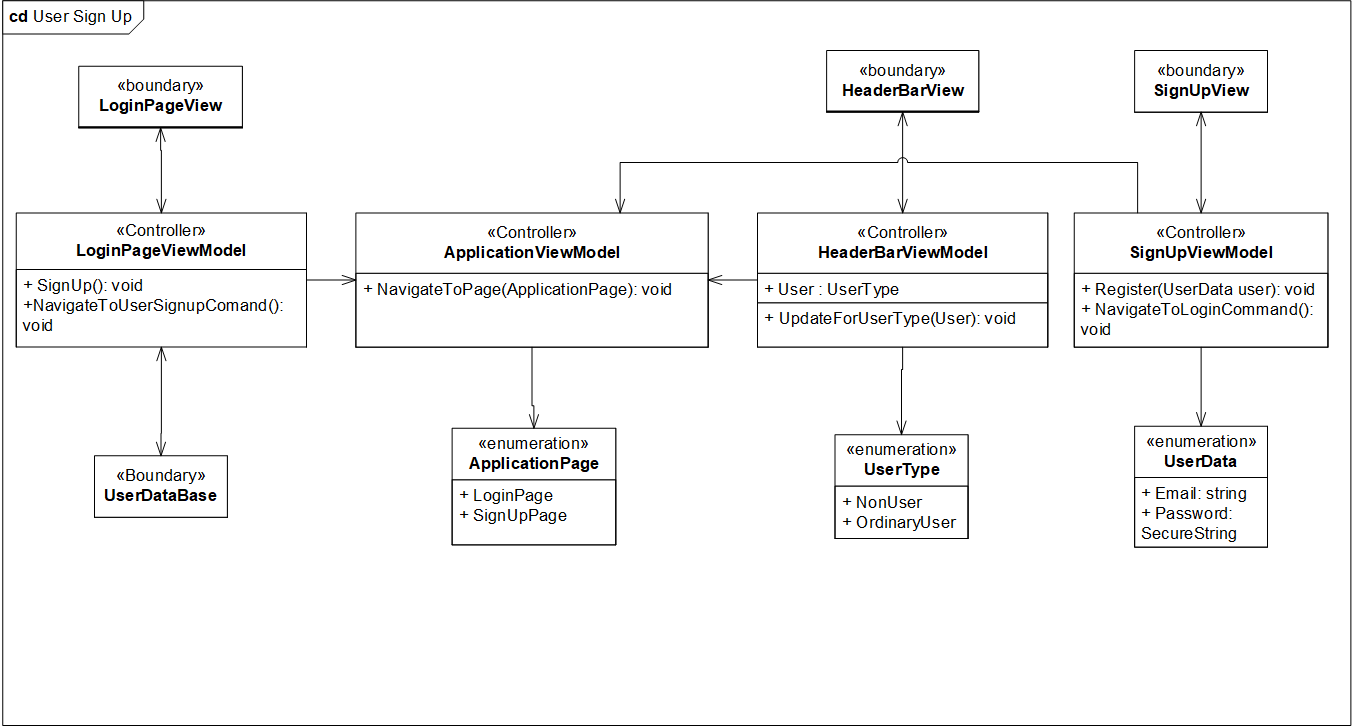
\includegraphics[width=\textwidth]{Arkitektur/Softwarearkitektur/User_Signup/graphics/UserSignUpCD.png}
    \caption{Klassediagram for oprettelse af bruger profil. }
    \label{fig:UserSignUpCD}
\end{figure}


\begin{figure}[H]
    \centering
    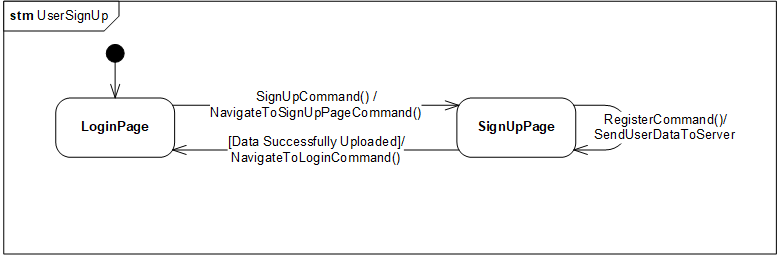
\includegraphics[width=\textwidth]{Arkitektur/Softwarearkitektur/User_Signup/graphics/UserSignUpSTM.png}
    \caption{Statemachine for oprettelse af bruger profil. }
    \label{fig:UserSignUpSTM}
\end{figure}

%BRUGERLOGIN
\subsubsection{Brugerlogin}
Når en bruger har lavet en bruger profil skal han herefter logge ind for at kunne udleje sin bil gennem applikationen eller leje en bil fra en udlejer. Til at beskrive denne funktionalitet er der lavet et klassediagram og en statemachine, som kan ses nedenfor. På figur \ref{fig:LoginCD} ses klassediagrammet og på figur \ref{fig:LoginSTM} ses statemachine.

\begin{figure}[H]
    \centering
    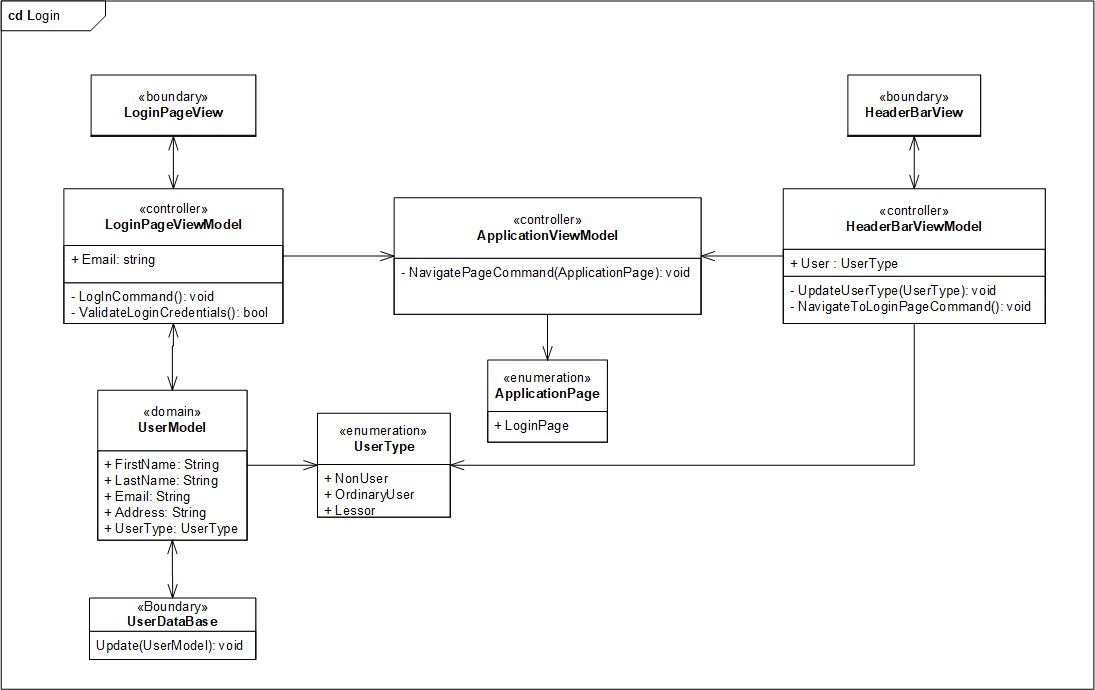
\includegraphics[width=\textwidth]{Arkitektur/Softwarearkitektur/User_Login/graphics/LoginCD.png}
    \caption{Klassediagram for bruger login. }
    \label{fig:LoginCD}
\end{figure}

\begin{figure}[H]
    \centering
    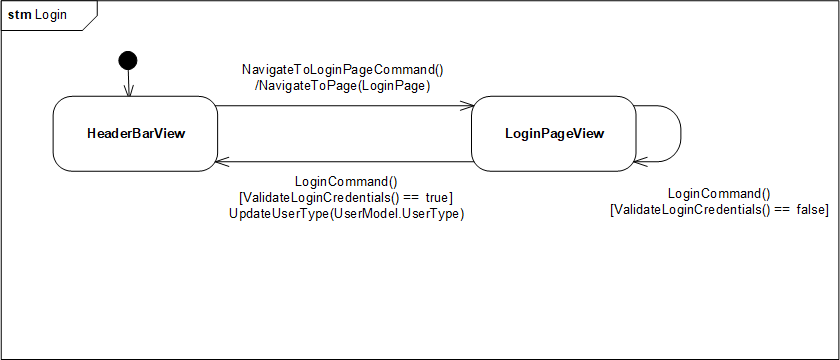
\includegraphics[width=\textwidth]{Arkitektur/Softwarearkitektur/User_Login/graphics/LoginSTM.png}
    \caption{Statemachinediagram for bruger login. }
    \label{fig:LoginSTM}
\end{figure}

%REDIGER AF BRUGERPROFIL
\subsubsection{Redigering af brugerprofil}
Når man som bruger har oprettet en profil, kan det være at ens oplysninger ændrer sig eller man har lavet en fejl. Den logiske arkitektur for dette kan ses på figur \ref{fig:EditUserCD} vises et klassediagram og på figur \ref{fig:EditUserSTM} vises et statemachine diagram.
\begin{figure}[H]
    \centering
    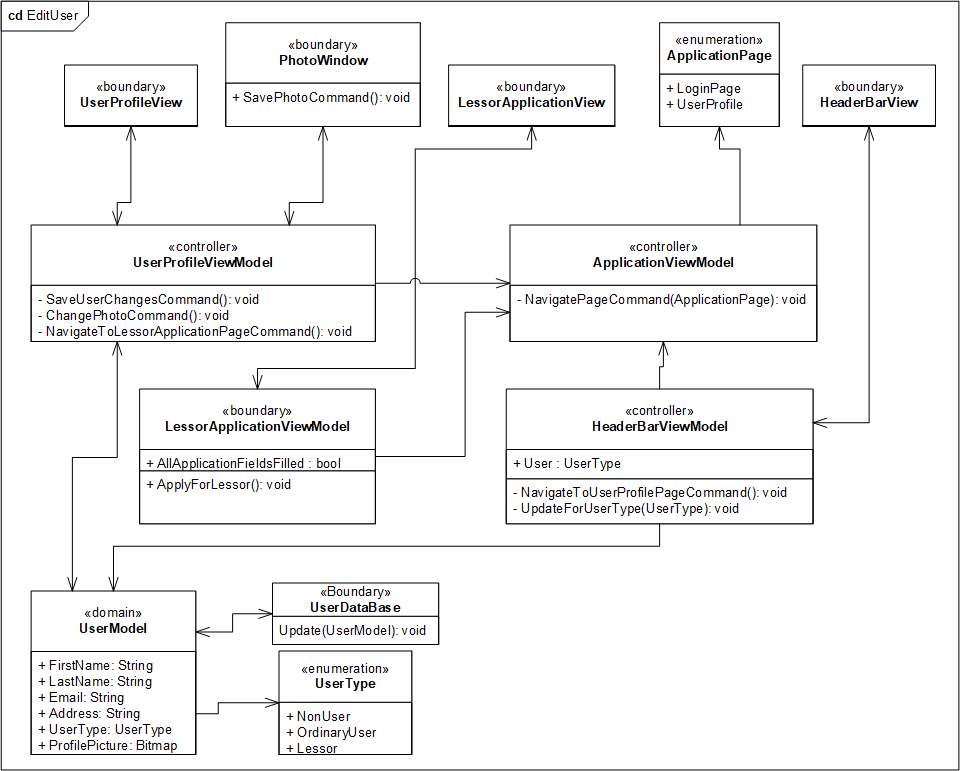
\includegraphics[width=1\textwidth]{Arkitektur/Softwarearkitektur/Edit_user_profile/graphics/EditUserCD.png}
    \caption{Klassediagram for redigering og fjernelse af en brugerprofil. }
    \label{fig:EditUserCD}
\end{figure}

\begin{figure}[H]
    \centering
    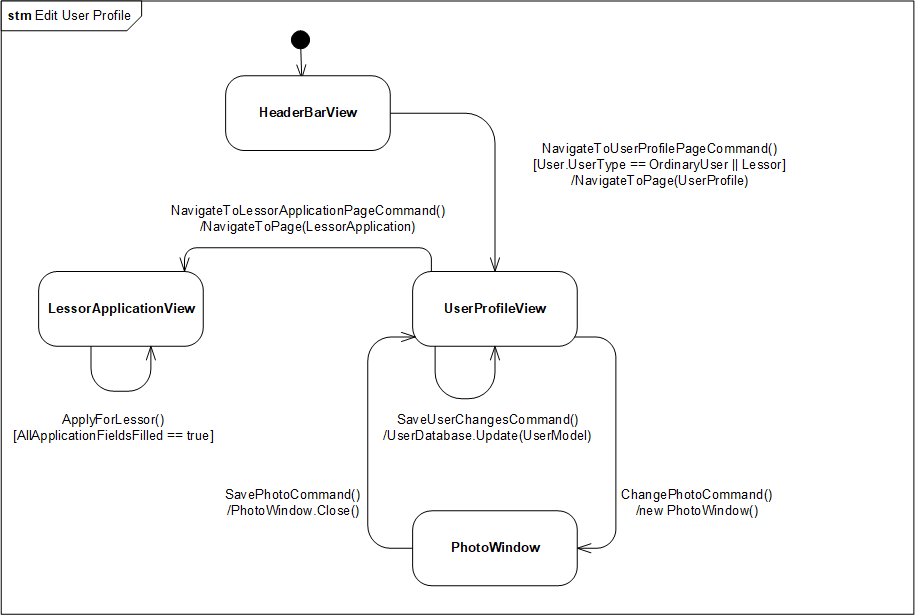
\includegraphics[width=1\textwidth]{Arkitektur/Softwarearkitektur/Edit_user_profile/graphics/EditUserSTM.png}
    \caption{Statemachine for redigering og fjernelse af en brugerprofil. }
    \label{fig:EditUserSTM}
\end{figure}

%REGISTRERING AF BILPROFIL
\subsubsection{Registrering af bilprofil}
Der er også lavet en applikationsmodel, som består af et klassediagram, som ses på figur \ref{fig:RegisterCarProfileCD}, og et statemachine diagram, som ses på figur \ref{fig:RegisterCarProfileSTM}.
\begin{figure}[H]
    \centering
    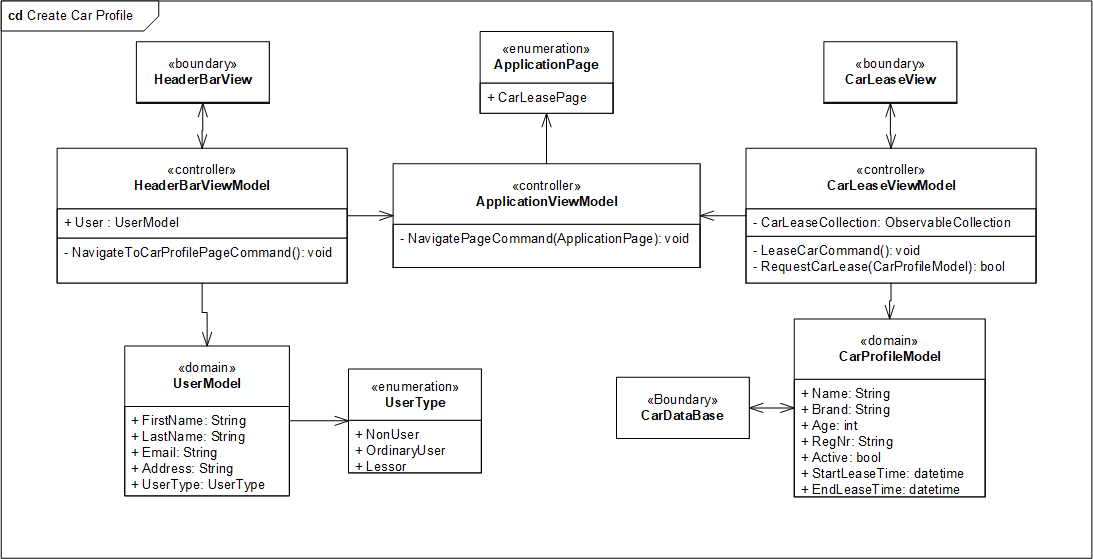
\includegraphics[width=1\textwidth]{Arkitektur/Softwarearkitektur/Car_registration/graphics/RegisterCarProfileCD.png}
    \caption{Her ses klassediagrammet for tilføjelse af bil til en brugerprofil. }
    \label{fig:RegisterCarProfileCD}
\end{figure}

\begin{figure}[H]
    \centering
    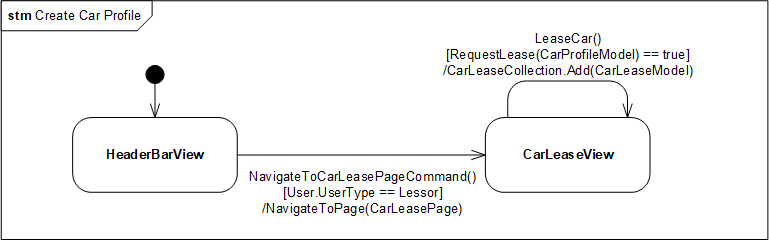
\includegraphics[width=1\textwidth]{Arkitektur/Softwarearkitektur/Car_registration/graphics/RegisterCarProfileSTM.png}
    \caption{Her ses Statemachinediagram for tilføjelse af bil til en brugerprofil. }
    \label{fig:RegisterCarProfileSTM}
\end{figure}

%FJERNELSE AF BILPROFIL
\subsubsection{Fjernelse af bilprofil}
Når en bruger ikke længere ønsker at udleje sin bil, så skal brugeren slette bilprofilen. Arkitekturen for denne funktionalitet er beskrevet med et klassediagram et klassediagram på figur \ref{fig:RemoveDeactivateCarProfileCD} og et statemachine diagram, som ses på figur \ref{fig:RemoveDeactivateCarProfileSTM}.
\begin{figure}[H]
    \centering
    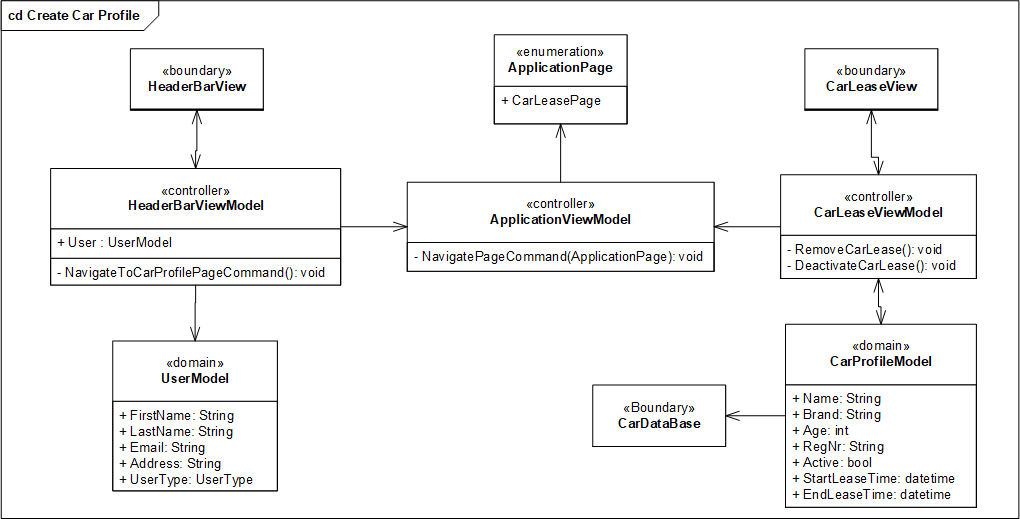
\includegraphics[width=1\textwidth]{Arkitektur/Softwarearkitektur/Car_registration/graphics/RemoveDeactivateCarProfileCD.png}
    \caption{Her ses klassediagrammet for fjernelse af bil fra en brugerprofil. }
    \label{fig:RemoveDeactivateCarProfileCD}
\end{figure}

\begin{figure}[H]
    \centering
    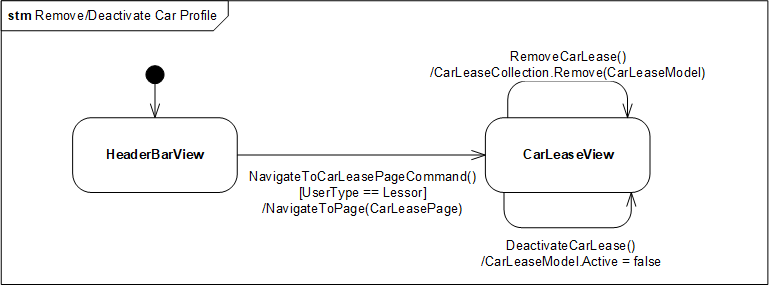
\includegraphics[width=1\textwidth]{Arkitektur/Softwarearkitektur/Car_registration/graphics/RemoveDeactivateCarProfileSTM.png}
    \caption{Her ses statemachine for fjernelse af bil fra en brugerprofil. }
    \label{fig:RemoveDeactivateCarProfileSTM}
\end{figure}

\subsubsection{Søgning efter bilprofil}
Når en lejer ønsker at leje en bil, så skal han søge efter en i applikationens katalog, hvor udlejer har sat dem til leje. Søgningsprocesen er først beskrevet med et klassediagram, som ses på figur \ref{fig:SearchProcessCD}, og et statemachine diagram, der ses på figur \ref{fig:SearchProcessSTM}.
\begin{figure}[H]
    \centering
    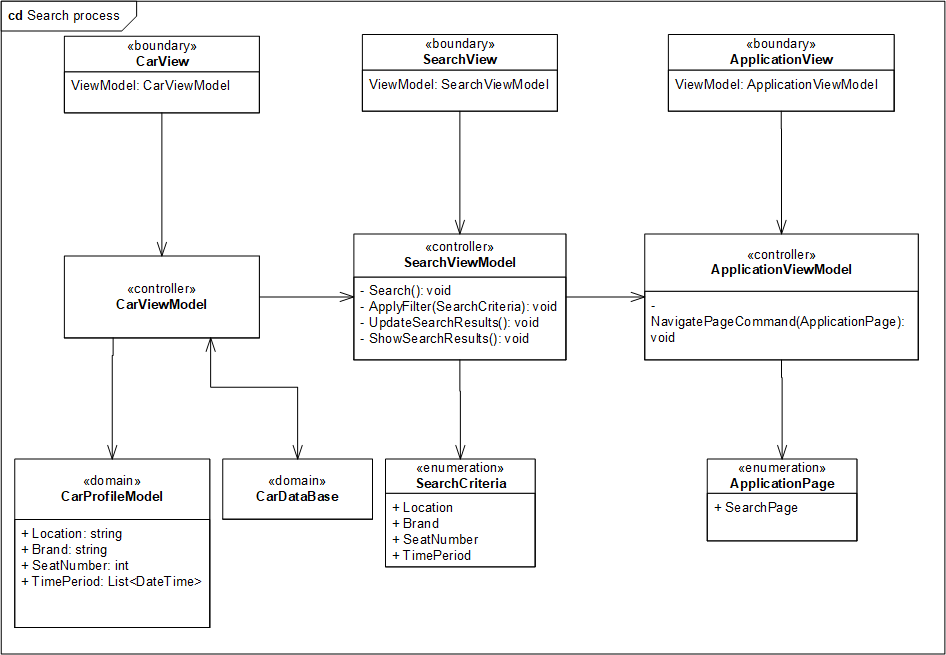
\includegraphics[width=1\textwidth]{Arkitektur/Softwarearkitektur/Searching/graphics/SearchProcessCD.png}
    \caption{Klassediagram for søgning efter biler til leje. }
    \label{fig:SearchProcessCD}
\end{figure}

\begin{figure}[H]
    \centering
    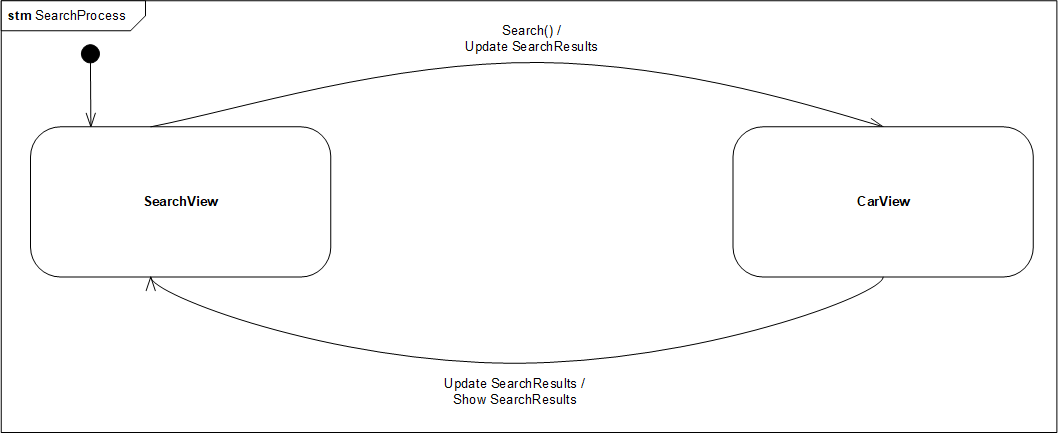
\includegraphics[width=1\textwidth]{Arkitektur/Softwarearkitektur/Searching/graphics/SearchProcessSTM.png}
    \caption{Statemachine for søgning efter biler til leje. }
    \label{fig:SearchProcessSTM}
\end{figure}

\subsubsection{Håndtering af udlejningsproces}
Efter at lejer har søgt i applikationens katalog, og har fundet en bil, som lejer ønsker at leje, så starter udlejningsprocessen. Nedenfor ses et klassediagram på figur \ref{fig:Leasing_processCD} og et statemachinediagram på figur \ref{fig:Leasing_processSTM}, der viser denne proces.
\begin{figure}[H]
    \centering
    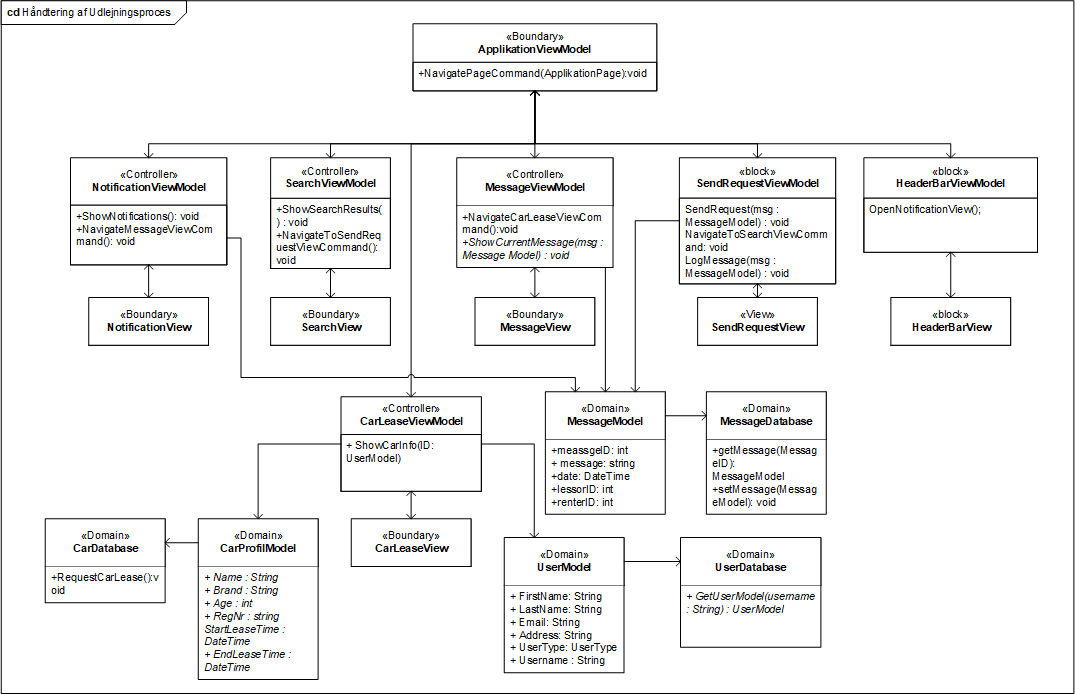
\includegraphics[width=1\textwidth]{Arkitektur/Softwarearkitektur/Leasing/graphics/Leasing_processCD.png}
    \caption{Klassediagram for håndtering af udlejningsprocessen.}
    \label{fig:Leasing_processCD}
\end{figure}

\begin{figure}[H]
    \centering
    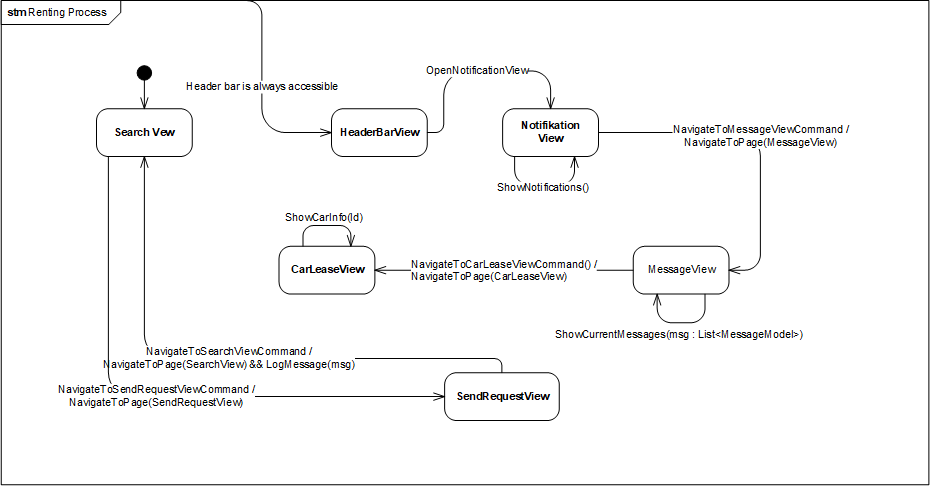
\includegraphics[width=1\textwidth]{Arkitektur/Softwarearkitektur/Leasing/graphics/Leasing_processSTM.png}
    \caption{Statmemachine for håndtering af udleningsprocessen. }
    \label{fig:Leasing_processSTM}
\end{figure}

\end{document}